\chapter{Perancangan}
\label{chap:perancangan}

Pada bab ini dijelaskan mengenai perancangan aplikasi yang dibangun meliputi perancangan
interaksi antar node, perancangan kelas aplikasi, perancangan format pesan, dan perancangan masukan dan keluaran.

\section{Perancangan Interaksi Antar Node}
\label{sec:41}
Berikut penjelasan lebih lanjut mengenai fungsi - fungsi aplikasi yang sudah dijelaskan pada analisis subbab \ref{subsec:analisisTopArs}.
 
\subsection{Diagram Sequence "Check Online Node"}
\begin{figure}[H]
	 
	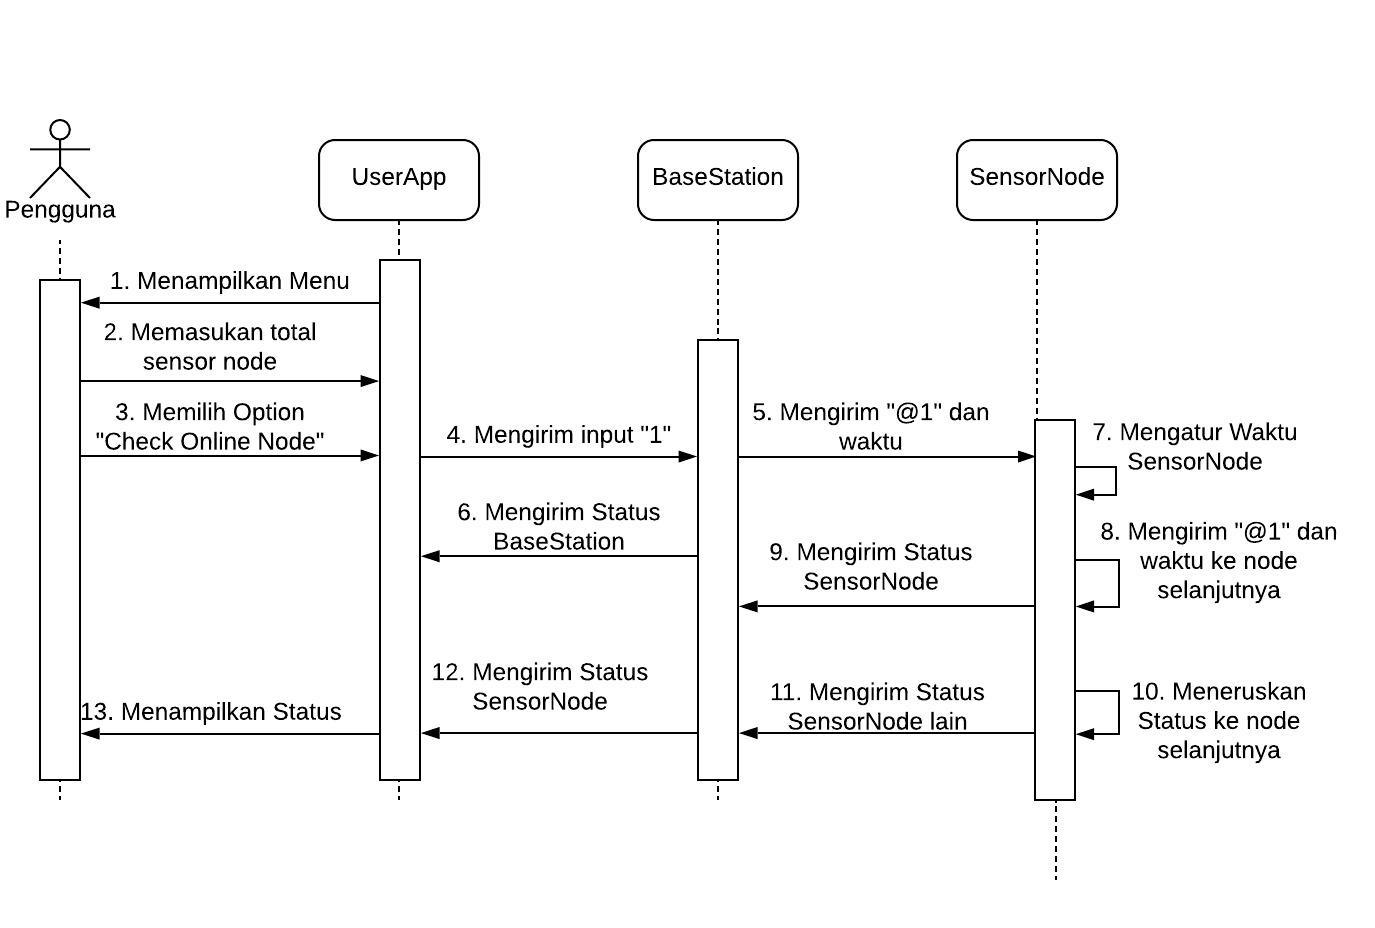
\includegraphics[scale=0.8]{checkOnlineNode}  
	\caption[Diagram sequence "Check Online Node"]{Diagram sequence "Check Online Node"} 
	\label{fig:checkOnlineNode} 
\end{figure} 

Pertama UserApp akan menampilkan menu untuk memasukkan total sensor node. Setelah pengguna memasukkan total sensor node, UserApp akan menampilkan menu fungsi - fungsi yang ada di aplikasi. Kemudian pengguna memilih option menu "Check Online Node". Fungsi Check Online Node digunakan untuk menyamakan waktu setiap sensor node dan {\it base station} dengan komputer pengguna dan menampilkan status online dari sensor node dan {\it base station}. Saat fungsi "Check Online Node" UserApp akan mengirim kode perintah "1" kepada BaseStation. Saat BaseStation menerima kode perintah "1", BaseStation akan mengirim kode perintah "@1" ke alamat sensor node yang tersimpan. Setiap SensorNode yang menerima kode perintah "@1" akan meneruskan perintah tersebut ke SensorNode selanjutnya dan mengirim status onlinenya ke BaseStation secara langsung atau melewati SensorNode lain. Jika BaseStation menerima status online dari SensorNode maka BaseStation akan meneruskan status tersebut ke UserApp dan UserApp akan menampilkan status online SensorNode tersebut.  
		
\subsection{Diagram Sequence "Sense"}
\begin{figure}[H]
	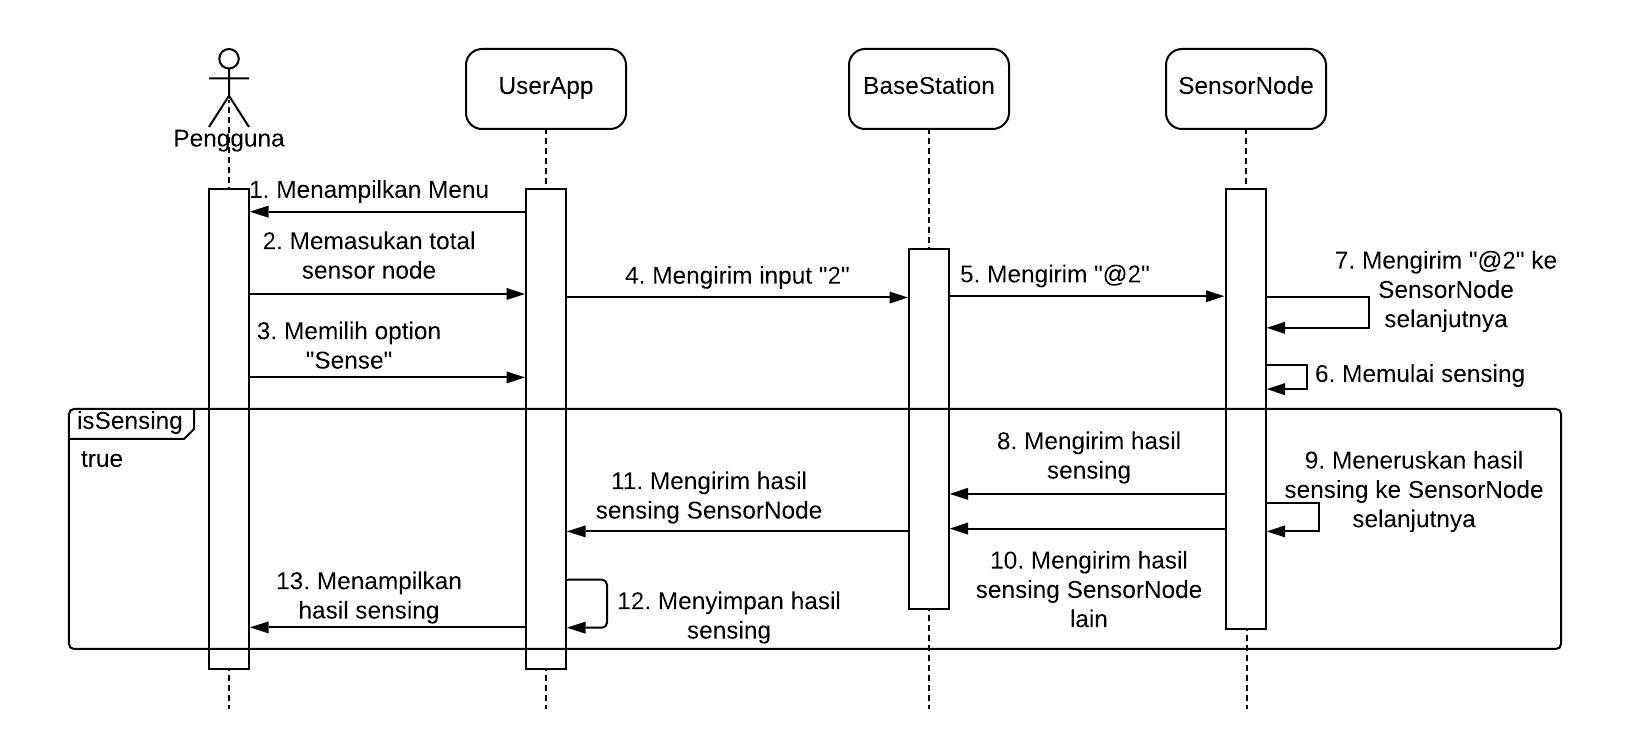
\includegraphics[scale=0.7]{sense}  
	\caption[Diagram sequence "Sense"]{Diagram sequence "Sense"} 
	\label{fig:sense} 
\end{figure} 

Pertama UserApp akan menampilkan menu untuk memasukkan total sensor node. Setelah pengguna memasukkan total sensor node, UserApp akan menampilkan menu fungsi - fungsi yang ada di aplikasi. Setelah Pengguna memilih option menu "Check Online Node", kemudian pengguna memilih option menu "Sense". Saat pengguna memilih option menu "Sense", UserApp akan mengirim kode perintah "2" ke BaseStation dan menampilkan grafik hasil sense. Setelah BaseStation menerima kode perintah "2" dari UserApp, BaseStation mengirim kode perintah "@2" ke alamat sensor node yang tersimpan. Setiap SensorNode yang menerima kode perintah "@2" akan mulai melakukan {\it sensing} dan meneruskan perintah tersebut ke SensorNode selanjutnya. Setiap hasil {\it sensing} dikirimkan ke BaseStation / SensorNode lain hingga sampai ke BaseStation. Hasil sensing yang diterima oleh BaseStation akan dikirim ke UserApp. Hasil sense akan langsung ditampilkan oleh UserApp dan disimpan dalam file oleh UserApp.

\subsection{Diagram Sequence "Stop Sensing"}
\begin{figure}[H]
	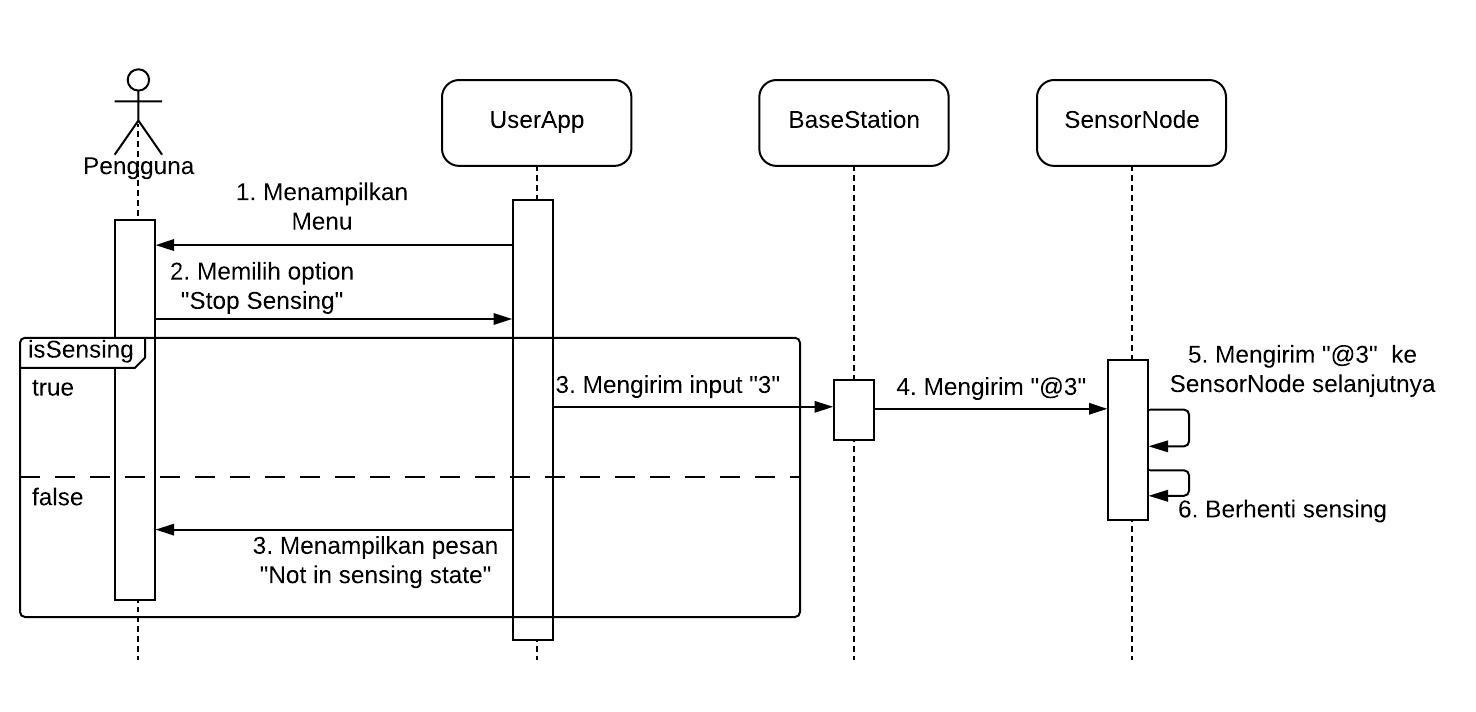
\includegraphics[scale=0.6]{stopSensing}  
	\caption[Diagram sequence "Stop Sensing"]{Diagram sequence "Stop Sensing"} 
	\label{fig:stopSensing} 
\end{figure} 

Pertama UserApp akan menampilkan fungsi - fungsi aplikasi. Kemudian pengguna memilih option menu "Stop Sensing". Jika SensorNode tidak sedang dalam keadaan "Sensing" maka UserApp akan menampilkan pesan "Sensor Node not in sensing state". Jika SensorNode sedang dalam keadaan sensing maka UserApp akan mengirim perintah "3" ke BaseStation. Saat kode perintah "3" diterima, BaseStation akan mengirim kode perintah "@3" ke alamat SensorNode yang tersimpan. Setiap SensorNode yang menerima kode perintah "@3" akan berhenti melakukan "sensing" dan meneruskan perintah ke SensorNode selanjutnya. Saat semua SensorNode berhenti melakukan "Sensing" UserApp akan menutup grafik hasil sense dan mengampilkan pesan "Stop Sensing Done". 

\subsection{Diagram Sequence "Exit"}
\begin{figure}[H]
	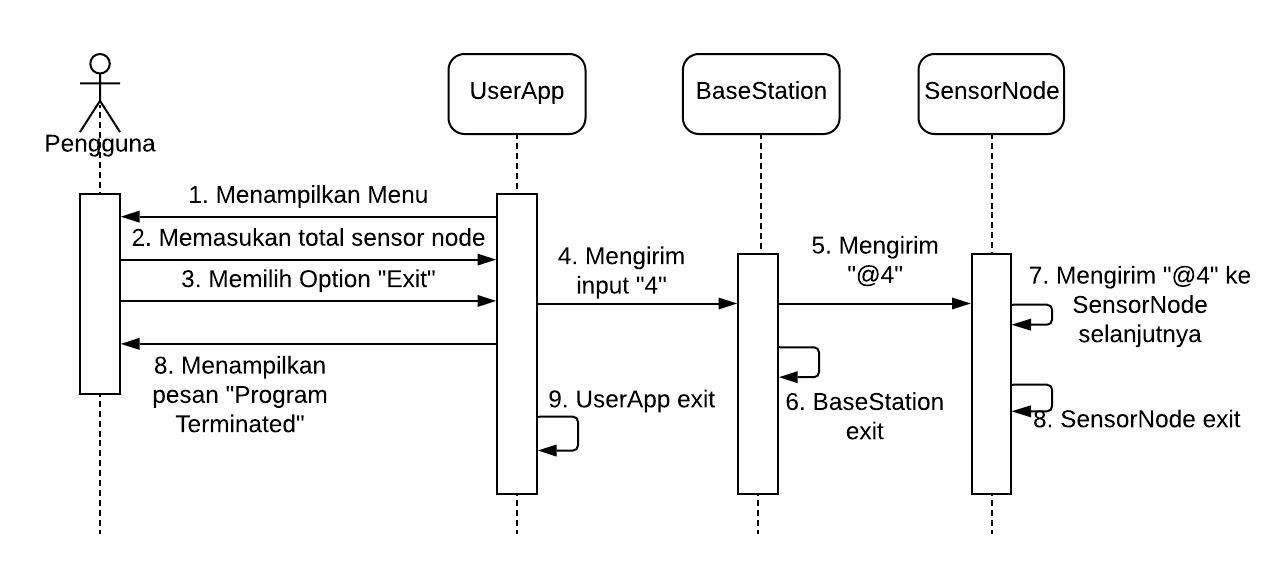
\includegraphics[scale=0.8]{exit}  
	\caption[Diagram sequence "Exit"]{Diagram sequence "Exit"} 
	\label{fig:exit} 
\end{figure} 

Pertama UserApp akan menampilkan menu untuk memasukkan total sensor node. Setelah pengguna memasukkan total sensor node, UserApp akan menampilkan menu fungsi - fungsi yang ada di aplikasi. Kemudian pengguna memilih option menu "Exit". Saat pengguna memilih option menu "Exit", UserApp akan mengirim perintah "4" ke BaseStation untuk mematikan program pada BaseStation. Saat kode perintah "4" diterima, BaseStation mengirim kode perintah "@4" ke alamat SensorNode yang tersimpan. SensorNode yang menerima kode perintah "@4" akan memberhentikan program dan meneruskan kode perintah ke SensorNode selanjutnya.

\section{Perancangan Antar Muka Untuk Visualisasi Hasil Ekstraksi}
Pada Subbab \ref{subsec:analisisFungsi} telah dijelaskan bahwa terdapat fungsi untuk menampilkan hasil sense. Perancangan antar muka ini memanfaatkan library JFreeChart \footnote{http://www.jfree.org/jfreechart/}. Berikut perancangan antar muka untuk tampilan hasil ekstraksi fitur.
\subsection{Antar Muka Visualisasi Hasil Sense }
\begin{figure}[H]
	\centering
	\includegraphics[scale=0.8]{Mockup/Visualizing}  
	\caption[Rancangan antar muka tampilan hasil sense]{Rancangan antar muka tampilan hasil sense} 
	\label{fig:MockupVisualizing} 
\end{figure} 
Keterangan Gambar : 
\begin{itemize}
	\item Nomor 1 : Judul dari visualisasi berdasarkan nama sensor
	\item Nomor 2 : label 'Amplitude' untuk sumbu $y$
	\item Nomor 3 : label 'Time' pada sumbu $x$
	\item Nomor 4 : Grafik plot dari hasil sense
	\item Nomor 5 : Keterangan plot pada grafik yang ditampilkan.
\end{itemize}

\subsection{Antar Muka Spectrogram}
\begin{figure}[H]
	\centering
	\includegraphics[scale=0.8]{Mockup/Spectrogram}  
	\caption[Rancangan antar muka tampilan hasil sense]{Rancangan antar muka tampilan hasil sense} 
	\label{fig:MockupVisualizing} 
\end{figure} 
Keterangan Gambar : 
\begin{itemize}
	\item Nomor 1 : Judul dari spectrogram berdasarkan nama sensor
	\item Nomor 2 : Grafik plot dari hasil ekstraksi fitur sensor node
	\item Nomor 3 : label 'Frequency' pada sumbu $y$
	\item Nomor 4 : label 'Amplitude' pada sumbu $z$ berupa skala perubahan warna 
	\item Nomor 5 : label 'Time (ms)' pada sumbu $x$
\end{itemize}

\section{Perancangan Kelas Aplikasi}
Pada Subbab \ref{subsec:analisisKelas} telah dijelaskan kelas diagram sederhana untuk fungsi - fungsi aplikasi ini. Berikut kelas diagram lengkap
dan detil kelas dari package {\it UserApp}, {\it BaseStation}, dan {\it SensorNode}

\subsection{Package UserApp}
Package ini berisi kelas {\it Tester} , kelas {\it Plotting}, kelas {\it Visualizing}, dan kelas {\it Spectrogram}.

\begin{figure}[H]
	\centering
	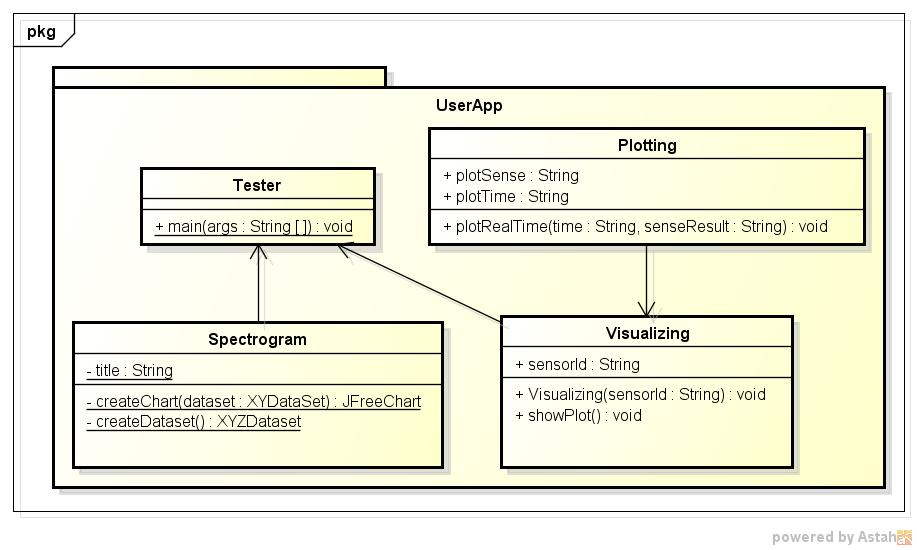
\includegraphics[scale=0.25]{KelasDiagramLengkap/UserApp}  
	\caption[Kelas diagram lengkap package UserApp]{Kelas diagram lengkap package UserApp} 
	\label{fig:KelasDiagramLengkapUserApp} 
\end{figure} 

\subsubsection{Kelas Tester}
\begin{figure}[H]
	\centering
	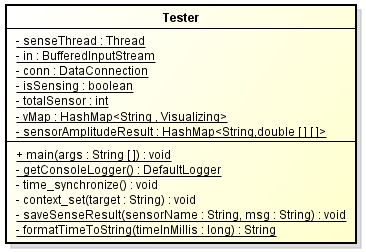
\includegraphics[scale=1.5]{KelasDiagram/Tester}  
	\caption[Perancangan Kelas Tester]{Perancangan Kelas Tester} 
	\label{fig:KelasTester} 
\end{figure} 

\newpage
Kelas ini digunakan sebagai main class yang menerima input dari pengguna dan menampilkan output ke pengguna. Atribut - atribut yang ada pada kelas ini adalah sebagai berikut:
\begin{itemize}
	\item private static Thread senseThread; \\
		Atribut ini digunakan untuk membuat {\it thread} baru yang bertugas menerima hasil sense dari sensor node saat dalam keadaan {\it sensing}.
	\item private static BufferedInputStream in; \\
		Atribut ini digunakan untuk membaca input dari BaseStation.
	\item private static DataConnection conn; \\
		Atribut ini digunakan untuk membuat koneksi dengan BaseStation.
	\item private static volatile boolean isSensing; \\
		Atribut ini digunakan untuk sebagai penanda kondisi SensorNode. Jika SensorNode dalam keadaan {\it sensing} maka atribut ini akan bernilai {\it true}.
	\item private static int totalSensor; \\
		Atribut ini digunakan untuk inisialisasi jumlah plot Visualizing dan Spectrogram sesuai dengan jumlah sensor yang digunakan.
	\item private static HashMap <String,Visualizing> vMap; \\
		Atribut ini digunakan untuk menyimpan objek - objek Visualizing pada HashMap.
	\item private static HashMap<String, double[][]> sensorAmplitudeResult; \\
		Atribut ini digunakan untuk menyimpan hasil dari ekstraksi fitur dari sensor node - sensor node ke dalam sebuah HashMap.
\end{itemize}
Metode - metode yang ada pada ini adalah sebagai berikut:
\begin{itemize}
	\item public static void main(String[] args) \\
		Metode ini digunakan sebagai metode main dari kelas ini. 
	\item private static DefaultLogger getConsoleLogger()\\
		Metode ini digunakan untuk memunculkan tulisan pada {\it console}.
	\item private void time\_ synchronize() \\
		Metode ini digunakan untuk mengatur dan memperbaharui waktu pada BaseStation dengan waktu pada komputer pengguna.
	\item private void context\_ set(String target)\\
		Metode ini digunakan untuk memilih {\it context} dari BaseStation
	\item private static void saveSenseResult(String sensorName, String msg) \\
		Metode ini digunakan untuk menyimpan semua hasil sensing ke dalam file.
	\item private static String formatTimetoString(long timeInMillis) \\
		Metode ini digunakan untuk mengubah format waktu dalam milli menjadi sebuah {\it string}.
\end{itemize}


\subsubsection{Kelas Plotting}
\begin{figure}[H]
	\centering
	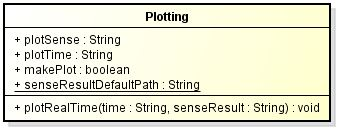
\includegraphics[scale=1.3]{KelasDiagram/Plotting}  
	\caption[Perancangan Kelas Plotting]{Perancangan Kelas Plotting} 
	\label{fig:KelasPlotting} 
\end{figure}
Kelas ini bertugas untuk menyimpan nilai waktu dan nilai hasil sense untuk diperbaharui oleh kelas Visualizing dalam membuat plot dari hasil {\it sensing}. Atribut - atribut yang ada pada kelas ini adalah sebagai berikut:
\begin{itemize}
	\item public String plotTime; \\
		Atribut ini menyimpan nilai waktu untuk ditampilkan pada visualisasi. 
	\item public double plotSense; \\
		Atribut ini menyimpan nilai sense untuk ditampilkan pada visualisasi.
	\item public boolean makePlot; \\
		Atribut ini digunakan sebagai penanda pembuatan plot. Jika bernilai 
		{\it true} maka Visualizing akan menampilkan plot dari nilai yang tersimpan pada plotTime dan plotSense.
	\item public static String senseResultDefaultPath; \\
		Atribut ini menyimpan {\it directory path} penyimpanan data hasil 
		{\it sensing} di komputer pengguna.
		
\end{itemize}
Metode - metode yang ada pada ini adalah sebagai berikut:
\begin{itemize}
	\item public void plotRealTime(String time, String senseResult) \\
		Metode ini digunakan untuk menyimpan nilai waktu ke dalam atribut plotTime ,nilai hasil sense ke dalam atribut plotSense, dan memperbolehkan kelas Visualizing untuk memperbaharui visualisasi yang sedang ditampilkan. 
\end{itemize}

\subsubsection{Kelas Visualisizing}
\begin{figure}[H]
	\centering
	\includegraphics[scale=1.3]{KelasDiagram/Visualizing}  
	\caption[Perancangan Kelas Visualizing]{Perancangan Kelas Visualizing} 
	\label{fig:KelasVisualizing} 
\end{figure}
Kelas ini bertugas untuk membuat dan menampilkan plot dari Kelas Plotting. Kelas ini akan terus memperbaharui plot yang sedang ditampilkan saat melakukan {\it sensing}. Atribut - atribut yang ada pada kelas ini adalah sebagai berikut:
\begin{itemize}
	\item public static volatile boolean canPlot; \\
		Atribut ini digunakan sebagai penanda dapat plot atau tidak
	\item public boolean showed; \\
		Atribut ini digunakan sebagai penanda sudah ditampilkan atau belum
	\item public final Plotting plotMaker = new Plotting(); \\
		Atribut ini digunakan untuk membuat objek Plotting 
	\item public JFrame frame;\\
		Atribut ini digunakan untuk menampung object JFrame
	\item public JFreeChart chart; \\
		Atribut ini digunakan untuk menampung object JFreeChart yang 
	\item public XYPlot plot; \\
		Atribut ini digunakan untuk mengatur plot yang divisualisasikan
	\item public String sensorId; \\
		Atribut ini digunakan untuk menyimpan SensorId 
	\item private TimeSeries amplitude; \\
		Atribut ini digunakan untuk membuat plot time series dari amplitude
	\item private TimeSeries frequency; \\
		Atribut ini digunakan untuk membuat plot time series dari frequency
\end{itemize}
Metode - metode yang ada pada kelas ini adalah sebagai berikut:
\begin{itemize}
	\item Visualizing(String sensorId) \\
		Metode ini digunakan sebagai konstruktor dari Kelas Visualizing
	\item private void addAmplitudeObservation(long milis, double y)
		Metode ini digunakan untuk menambahkan plot amplitude pada grafik
	\item private void addFreqObservation(long milis, double y) 
		Metode ini digunakan untuk menambahkan plot frequency pada grafik
\end{itemize}
Pada kelas ini terdapat {\it inner class} DataGenerator yang memiliki atribut :
\begin{itemize}
	\item private Long lastTime = new Long(0);\\
		Atribut ini digunakan sebagai penanda waktu terakhir
\end{itemize}
kelas ini juga memiliki metode - metode sebagai berikut:
\begin{itemize}
	\item DataGenerator(int interval) \\
		Metode ini digunakan sebagai konstruktor dari kelas DataGenerator
	\item public void actionPerformed(ActionEvent event) \\
		Metode ini digunakan sebagai aksi yang dilakukan dalam interval tertentu
	\item public void showPlot()\\
		Metode ini digunakan untuk menampilkan plot pada tampilan
\end{itemize}

\subsubsection{Kelas Spectrogram}
\begin{figure}[H]
	\centering
	\includegraphics[scale=1]{KelasDiagram/Spectrogram}  
	\caption[Perancangan Kelas Spectrogram]{Perancangan Kelas Spectrogram} 
	\label{fig:KelasSpectrogram} 
\end{figure}
Kelas ini bertugas untuk membuat plot berupa Spectrogram yang menampilkan hasil  ekstraksi fitur dari sensor node. Atribut - atribut yang ada pada kelas ini adalah sebagai berikut:
\begin{itemize}
	\item private static double maxAmp;\\
		Atribut ini menyimpan amplitudo maksimal dari hasil ekstraksi fitur sensor node. 
	\item private static int length;\\
		Atribut ini menyimpan panjang dari hasil ekstraksi fitur sensor node.
	\item private static double[][] resAmplitude;\\
		Atribut ini menyimpan hasil dari ekstraksi fitur sensor node.
	\item private static double[] resTime;\\
		Atribut ini menyimpan waktu dari ekstraksi fitur.
	\item private static double fs;\\
		Atribut ini menyimpan {\it sampling frequency} dari ekstraksi fitur.
	\item private static int windowSize;\\
		Atribut ini menyimpan besar {\it window} yang digunakan oleh sensor node untuk ekstraksi fitur.
	\item private static double overlap;\\
		Atribut ini menyimpan nilai {\it overlap} yang digunakan oleh sensor node untuk ekstraksi fitur.
	\item private static String title;\\
		Atribut ini menyimpan judul dari Spectrogram.
	\item private static double deltaTime;\\
		Atribut ini meyimpan selisih waktu dari setiap hasil ekstraksi fitur.
\end{itemize}
Metode - metode yang ada pada kelas ini adalah sebagai berikut:
\begin{itemize}
	\item public Spectrogram(String title, double[][] resA, double[] resTime, double fs, int windowSize, double overlap,
			double deltaTime) \\
		Metode ini digunakan sebagai konstruktor dari kelas Spektrogram.
	\item private static JFreeChart createChart(XYDataset dataset) \\
		Metode ini berfungsi untuk membuat grafik spectrogram dari {\it dataset} yang sudah dibuat.
	\item private static XYZDataset createDataset()\\
		Metode ini berfungsi untuk membuat {\it dataset} dari hasil ekstrasi fitur sensor node.
\end{itemize}
Pada kelas ini terdapat {\it inner class} SpectrumPaintScale yang memiliki atribut - atribut sebagai berikut:
\begin{itemize}
	\item private final double lowerBound;\\
		Atribut ini digunakan untuk menyimpan nilai amplitudo terendah dari ekstraksi fitur.
	\item private final double upperBound;\\
		Atribut ini digunakan untuk menyimpan nilai amplitudo tertinggi dari hasil ekstraksi fitur.
\end{itemize}
Kelas ini juga memiliki metode - metode sebagai berikut: 
\begin{itemize}
	\item public SpectrumPaintScale(double lowerBound, double upperBound)\\
		Metode ini digunakan sebagai konstruktor dari kelas SpectrumPaintScale.
	\item public double getLowerBound()\\
		Metode ini mengembalikan nilai dari atribut lowerBound.
	\item public double getUpperBound() \\
		Metode ini mengembalikan nilai dari atribut upperBound.
	\item public Paint getPaint(double value)\\
		Metode ini mengembalikan objek {\it Paint} berdasarkan nilai {\it value} yang dibandingkan dengan atribut {\it lowerBound} dan {\it upperBound}.
\end{itemize}

\subsection{Package BaseStation}
Package ini berisi kelas {\it BSManager}.

\begin{figure}[H]
	\centering
	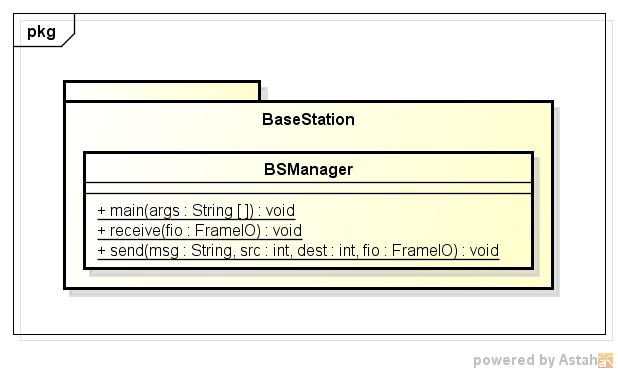
\includegraphics[scale=0.4]{KelasDiagramLengkap/BaseStation}  
	\caption[Kelas diagram lengkap package BaseStation]{Kelas diagram lengkap package BaseStation} 
	\label{fig:KelasDiagramLengkapBaseStation} 
\end{figure} 

\subsubsection{Kelas BSManager}
\begin{figure}[H]
	\centering
	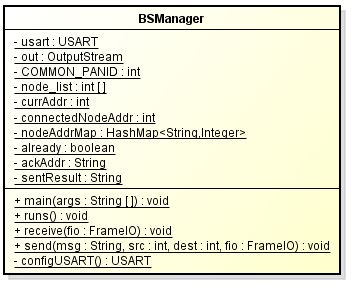
\includegraphics[scale=1.3]{KelasDiagram/BSManager}  
	\caption[Perancangan Kelas BSManager]{Perancangan Kelas BSManager} 
	\label{fig:KelasBSManager} 
\end{figure}
Kelas ini digunakan untuk sebagai main class dari package ini. Kelas ini akan berfungsi untuk menerima perintah dari UserApp, meneruskan perintah ke sensor node, menerima pesan dari sensor node, dan meneruskan pesan ke UserApp. Kelas ini memiliki atribut - atribut sebagai berikut :
\begin{itemize}
	\item private static USART usart;
		Atribut ini digunakan untuk mengatur usart pada BaseStation.
	\item private static OutputStream out;
		Atribut ini digunakan untuk mengatur outputstream ke UserApp.
	\item private static int COMMON\_ PANID;
		Atribut ini digunakan untuk mengatur panID.
	\item private static int[] node\_ list;
		Atribut ini menyimpan alamat - alamat dari sensor node.
	\item private static int currAddr = node\_ list[0];
		Atribut ini menyimpan alamat dari BaseStation.
	\item private static int[] connectedNodeAddr;
		Atribut ini menyimpan alamat - alamat sensor node yang terhubung dengan BaseStation.
	\item private static HashMap<String, Integer> nodeAddrMap;
		Atribut ini menyimpan alamat - alamat dari sensor node yang terhubung dengan BaseStation ke dalam HashMap.
	\item private static boolean already;
		Atribut ini digunakan untuk menunjukkan sudahnya SensorNode mengirim data.
	\item	private static String ackAddr;
		Atribut ini digunakan untuk menyimpan sensorId yang sedang mengirim data.
	\item private static String sentResult;
		Atribut ini digunakan untuk menyimpan data yang terkirim oleh sensor node.
		
\end{itemize}
Metode - metode yang ada pada ini adalah sebagai berikut:
\begin{itemize}
	\item public static void main(String[] args) \\
		Metode ini digunakan sebagai metode main kelas BSManager.
	\item public static void runs()\\
		Metode ini digunakan sebagai inisialisasi radio dan memulai {\it thread} untuk menerima dan mengirim pesan.
	\item public static void receive(final FrameIO fio) \\
		Metode ini digunakan untuk menerima pesan yang dikirim oleh sensor node.
	\item public static void send(String msg, int src, int dest, FrameIO fio) \\
		Metode ini digunakan untuk mengirim pesan ke sensor node.
	\item private static USART configUSART() \\
		Metode ini digunakan untuk inisialisasi usart.
\end{itemize}

\subsection{Package SensorNode}
Package ini berisi kelas {\it SNManager}, {\it Complex}, {\it FFT}, {\it ShortTimeFourierTransform}, {\it Accelerometer}, dan {\it SenseController}.

\begin{figure}[H]
	\centering
	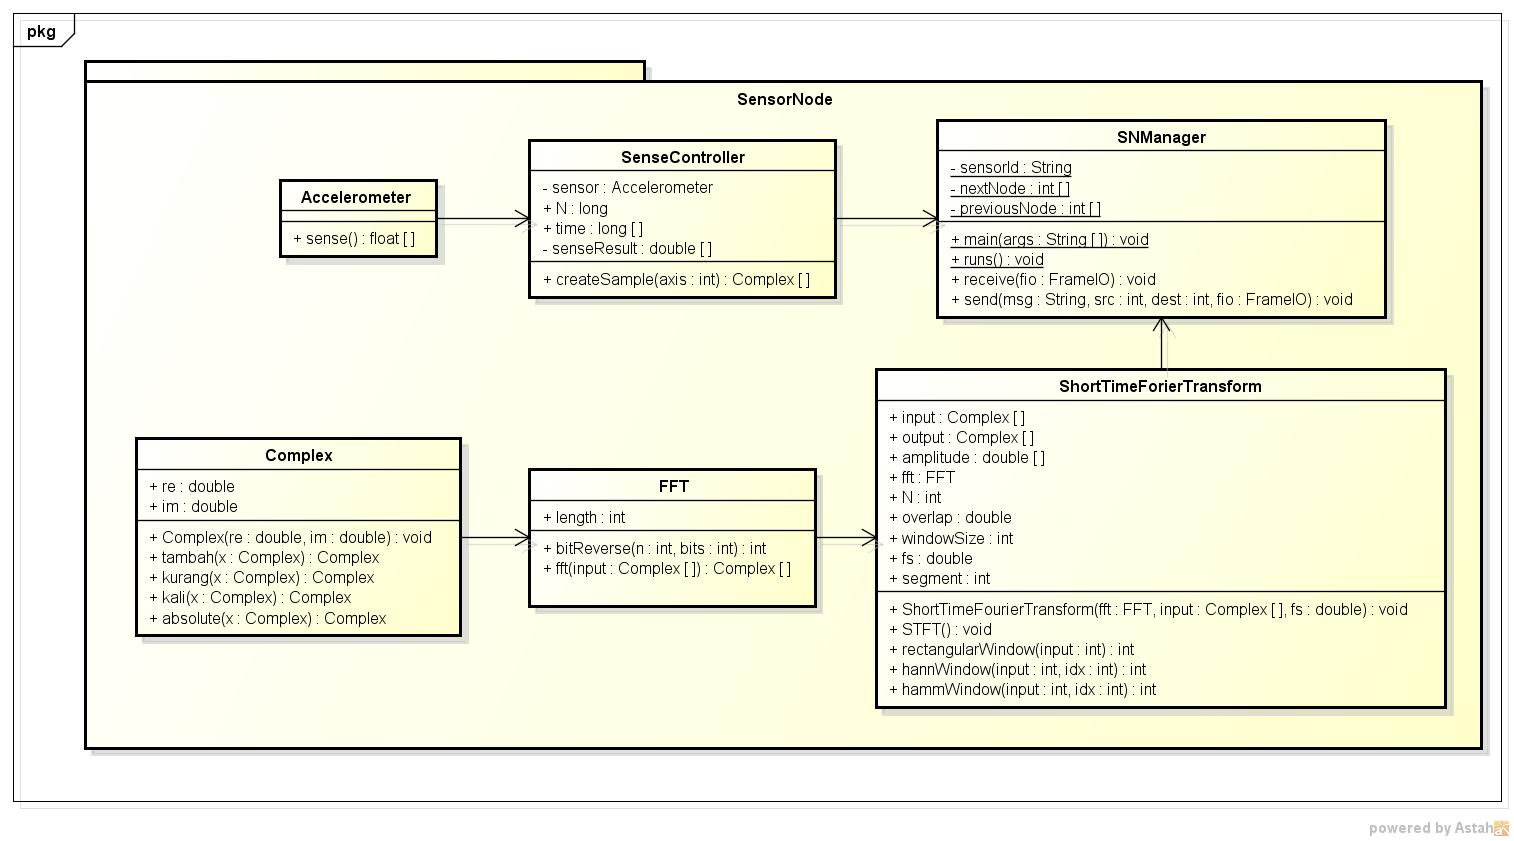
\includegraphics[scale=0.29]{KelasDiagramLengkap/SensorNode}  
	\caption[Kelas diagram lengkap package SensorNode]{Kelas diagram lengkap package SensorNode} 
	\label{fig:KelasDiagramLengkapSensorNode} 
\end{figure}  

\subsubsection{Kelas SNManager}
\begin{figure}[H]
	\centering
	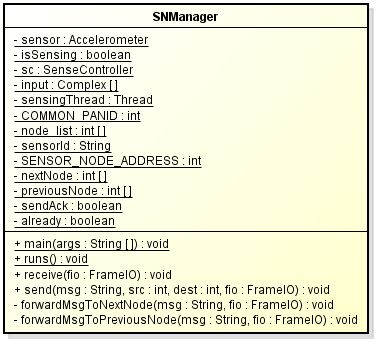
\includegraphics[scale=1.3]{KelasDiagram/SNManager}  
	\caption[Perancangan Kelas SNManager]{Perancangan Kelas SNManager} 
	\label{fig:KelasSNManager} 
\end{figure}

Kelas ini digunakan untuk sebagai main class dari package ini. Kelas ini akan berfungsi untuk menerima pesan dari sensor node lain, mengirim pesan ke sensor node yang terhubung, meneruskan pesan ke sensor node lain, dan mengirim hasil ekstraksi fitur ke BaseStation atau sensor node sebelumnya. Kelas ini memiliki atribut - atribut sebagai berikut :
\begin{itemize}
	\item private static final Accelerometer sensor  \\
		Atribut ini menyimpan objek kelas Accelerometer.
	\item private static boolean isSensing \\
		Atribut ini menandakan kondisi sensing SensorNode. Jika {\it isSensing} bernilai {\it true} maka SensorNode sedang dalam keadaan {\it sensing}. 
	\item private static SenseController sc\\
		Atribut ini menyimpan objek SenseController.
	\item private static Complex[] input; \\
		Atribut ini menyimpan input dari hasil {\it sensing} akselerometer.
	\item private static Thread sensingThread;\\
		Atribut ini digunakan untuk membuat {\it thread} baru untuk melakukan {\it sensing}.
	\item private static int COMMON\_ PANID \\
		Atribut ini menyimpan PanID.
	\item private static int[] node\_ list \\
		Atribut ini menyimpan alamat - alamat dari sensor node.
	\item private static final String sensorId \\
		Atribut ini menyimpan id dari sensor node.
	\item private static int SENSOR\_ NODE\_ ADDRESS \\
		Atribut ini menyimpan alamat sensor node dirinya sendiri.
	\item private static int[] nextNode \\
		Atribut ini menyimpan alamat - alamat dari sensor node selanjutnya.
	\item private static int[] previousNode \\
		Atribut ini menyimpan alamat - alamat dari sensor node sebelumnya
	\item private static boolean sendAck;\\
		Atribut ini digunakan sebagai penanda bahwa SensorNode dapat mengirim data ke BaseStation. Jika bernilai {\it true} maka sensor node dapat mengirim pesan ke BaseStation.
	\item private static boolean already; \\
		Atribut ini digunakan sebagai penanda bahwa SensorNode sudah mengirim data ke BaseStation. Jika bernilai {\it true} maka BaseStation sudah menerima data yang dikirim oleh sensor node.
\end{itemize}
Metode - Metode yang ada pada ini adalah sebagai berikut:
\begin{itemize}
	\item public static void main(String[] args) \\
		Metode ini digunakan sebagai metode main kelas BSManager.
	\item public static void runs()\\
		Metode ini digunakan sebagai inisialisasi radio dan memulai {\it thread} baru untuk menerima pesan dari BaseStation atau sensor node lain.
	\item public static void receive(final FrameIO fio) \\
		Metode ini digunakan untuk menerima pesan yang terkirim dan mengolah perintah yang diterima.
	\item public static void send(String msg, int src, int dest, FrameIO fio) \\
		Metode ini digunakan untuk mengirim pesan ke sensor node atau BaseStation.
	\item private static void forwardMsgToNextNode(String msg, FrameIO fio) \\
		Metode ini digunakan untuk meneruskan pesan ke sensor node selanjutnya.
	\item private static void forwardMsgToPreviousNode(String msg, FrameIO fio) \\
		Metode ini digunakan untuk meneruskan pesan ke sensor node sebelumnya.
\end{itemize}

\subsubsection{Kelas Complex}
\begin{figure}[H]
	\centering
	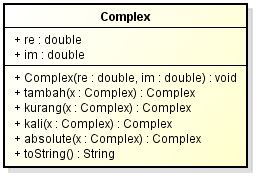
\includegraphics[scale=1.3]{KelasDiagram/Complex}  
	\caption[Perancangan Kelas Complex]{Perancangan Kelas Complex} 
	\label{fig:KelasComplex} 
\end{figure}

Kelas ini digunakan untuk sebagai objek yang merepresentasikan bilangan kompleks. Kelas ini memiliki atribut - atribut sebagai berikut :
\begin{itemize}
	\item public double re; \\
		Atribut ini digunakan untuk menyimpan bilangan real
    \item public double im; \\
    	Atribut ini digunakan untuk menyimpan bilangan imajiner
\end{itemize}
Metode - metode yang ada pada ini adalah sebagai berikut:
\begin{itemize}
	\item public Complex(double r, double i) \\
		Metode ini digunakan sebagai konstruktor dari kelas Complex.
    \item public Complex tambah(Complex x) \\
    	Metode ini digunakan untuk melakukan penjumlahan antar bilangan komplex.
    \item public Complex kurang(Complex x) \\
    	Metode ini digunakan untuk melakukan pengurangan antar bilangan komplex.
    \item public Complex kali(Complex x)\\
    	Metode ini digunakan untuk melakukan perkalian antar bilangan komplex.
    \item public double absolute()\\
    	Metode ini digunakan untuk mendapat amplitude dari bilangan kompleks.
    \item public String toString()\\
    	Metode ini digunakan untuk menjadikan objek bilangan komplex menjadi sebuah {\it string}.
\end{itemize}

\subsubsection{Kelas Accelerometer}
\begin{figure}[H]
	\centering
	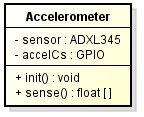
\includegraphics[scale=1.3]{KelasDiagram/Accelerometer}  
	\caption[Perancangan Kelas Accelerometer]{Perancangan Kelas Accelerometer} 
	\label{fig:KelasAccelerometer} 
\end{figure}

Kelas ini digunakan untuk mengatur dan menginisialisasi sensor akselerometer yang terdapat pada sensor node.. Kelas ini memiliki atribut - atribut sebagai berikut :
\begin{itemize}
	\item private ADXL345 sensor;
		Atribut ini digunakan sebagai objek driver untuk akselerometer ADXL345.
	\item private GPIO accelCs;
		Atribut ini digunakan sebagai objek GPIO.
\end{itemize}
Metode - metode yang ada pada ini adalah sebagai berikut:
\begin{itemize}
	\item public void init() \\
		Metode ini digunakan untuk menginisialisasi sensor akselerometer ADXL345.
	\item public float[] sense() \\
		Metode ini digunakan untuk mendapatkan data pengukuran akselerasi dari ADXL345.
\end{itemize}

\subsubsection{Kelas FFT}
\begin{figure}[H]
	\centering
	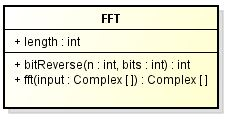
\includegraphics[scale=1.3]{KelasDiagram/FFT}  
	\caption[Perancangan Kelas FFT]{Perancangan Kelas FFT} 
	\label{fig:KelasFFT} 
\end{figure}

Kelas ini digunakan untuk melakukan komputasi FFT dari input bilangan complex . Kelas ini memiliki atribut sebagaii berikut:
\begin{itemize}
	\item public int length; \\
	Atribut ini menyimpan panjang dari algoritma FFT.
\end{itemize}
Metode - metode yang ada pada ini adalah sebagai berikut:
\begin{itemize}
	\item public int bitReverse(int n, int bits) \\
		Metode ini digunakan untuk melakukan bit reverse pada bilangan masukan. 
	\item public Complex [] fft(Complex[] input) \\
		Metode ini digunakan untuk melakukan komputasi FFT pada input yang dimasukkan. 
\end{itemize}

\subsubsection{Kelas ShortTimeFourierTransform}
\begin{figure}[H]
	\centering
	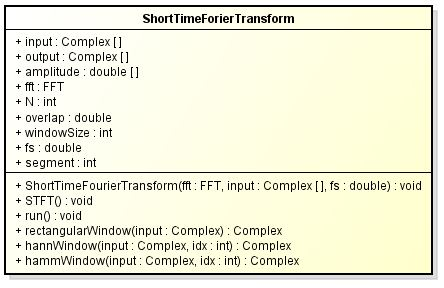
\includegraphics[scale=1.3]{KelasDiagram/ShortTimeFourierTransform}  
	\caption[Perancangan Kelas ShortTimeFourierTransform]{Perancangan Kelas ShortTimeFourierTransform} 
	\label{fig:KelasShortTimeFourierTransform} 
\end{figure}

Kelas ini digunakan untuk melakukan komputasi ShortTimeFourierTransform. Kelas ini memiliki atribut - atribut sebagai berikut :
\begin{itemize}
	\item private Complex [] input; \\
		Atribut ini digunakan untuk menyimpan input data hasil {\it sensing} akselerometer.
	\item public Complex [] output; \\
		Atribut ini digunakan untuk menyimpan output hasil STFT dari data input
	\item public double [] amplitude; \\
		Atribut ini digunakan untuk menyimpan hasil amplitudo dari output	
	\item public FFT fft; \\
		Atribut ini digunakan untuk menyimpan objek kelas FFT yang akan digunakan untuk komputasi STFT.
	\item public int N; \\
		Atribut ini digunakan untuk menyimpan besar {\it sample}.
	\item public double overlap = 0; \\
		Atribut ini menyimpan nilai overlap yang digunakan untuk komputasi algoritma STFT.
	\item public int windowSize;
		Atribut ini menyimpan panjang dari window yang digunakan untuk komputasi STFT.
	\item public double fs;  \\
		Atribut ini menyimpan nilai {\it sampling rate} dari {\it sensing}.
	\item public int segment; \\
		Atribut ini menyimpan banyak segment yang digunakan untuk komputasi algoritma STFT.
\end{itemize}
metode - metode yang ada pada ini adalah sebagai berikut:
\begin{itemize}
	\item public ShortTimeFourierTransform(FFT fft , Complex [] input, double fs) \\
		Metode ini digunakan sebagai konstruktor dari kelas ShortTimeFourierTransform.
	\item public void STFT() \\
		Metode ini digunakan untuk melakukan komputasi algoritma STFT pada input hasil {\it sensing}.
	\item public void run() \\
		Metode ini digunakan untuk memanggil metode STFT().
	\item public Complex rectangularWindow(Complex input) \\
		Metode ini digunakan untuk mengaplikasikan {\it Rectangular Window} pada input hasil {\it sensing}.
	\item public Complex hannWindow(Complex input, int idx) \\
		Metode ini digunakan untuk mengaplikasikan {\it Hanning Window} pada input hasil {\it sensing}.
	\item public Complex hammWindow(Complex input, int idx) \\
		Metode ini digunakan untuk mengaplikasikan {\it Hamming Window} pada input hasil {\it sensing}.
		
\end{itemize}

\subsubsection{Kelas SenseController}
\begin{figure}[H]
	\centering
	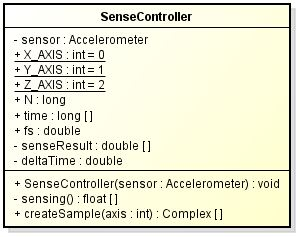
\includegraphics[scale=1.3]{KelasDiagram/SenseController}  
	\caption[Perancangan Kelas SenseController]{Perancangan Kelas SenseController} 
	\label{fig:KelasSenseController} 
\end{figure}

Kelas ini digunakan untuk mengatur pengukuran akselerometer dan membuat {\it sample} getaran. Kelas ini memiliki atribut - atribut sebagai berikut :
\begin{itemize}
	\item private Accelerometer sensor; \\
		Atribut ini digunakan sebagai objek Accelerometer
	\item public static final int X\_ AXIS = 0; \\
		Atribut ini digunakan sebagai input pada metode sensing().
	\item public static final int Y\_ AXIS = 1; \\
		Atribut ini digunakan sebagai input pada metode sensing().
	\item public static final int Z\_ AXIS = 2; \\
		Atribut ini digunakan sebagai input pada metode sensing().
	\item public final int N;  \\
		Atribut ini digunakan untuk menyimpan besar {\it sample}.
	\item public long [] time; \\
		Atribut ini digunakan untuk menyimpan waktu saat {\it sensing}.
	\item public double fs; \\
		Atribut ini digunakan untuk menyimpan {\it sampling rate}.
	\item public float [] senseResult; \\
		Atribut ini digunakan untuk menyimpan hasil {\it sensing} dari akselerometer untuk dijadikan {\it sample}.
	\item public double deltaTime;\\
		Atribut ini digunakan untuk menyimpan selisih waktu dari {\it sensing}.
\end{itemize}
metode - metode yang ada pada ini adalah sebagai berikut:
\begin{itemize}
	\item public SenseController(Accelerometer sensor) \\
		Metode ini digunakan sebagai konstruktor dari kelas ShortTimeFourierTransform
	\item private float[] sensing() \\
		Metode ini digunakan untuk melakukan sensing dengan Accelerometer
	\item public Complex[] createSample(int axis) \\
		Metode ini digunakan untuk membuat sample pada sumbu berdasarkan input 
\end{itemize}

\section{Perancangan Masukan dan Keluaran}
Aplikasi ini menggunakan {\it command line interface} untuk menerima input dan menampilkan keluaran dari aplikasi. Setiap masukan untuk aplikasi ini bertipe data {\it integer}. Aplikasi ini menampilkan 4 pilihan fungsi utama (\ref{sec:41}) dan pengguna dapat memasukkan nilai 1 - 4 sebagai masukan. Berikut penjelasan mengenai tiap masukan yang dapat dimasukkan oleh pengguna.
\begin{itemize}
	\item Masukan dengan nilai 1 / "Check Online Node" digunakan untuk mengetahui status dari setiap sensor node dan memnyamakan waktu - waktu yang ada di sensor node
	\item Masukan dengan nilai 2 / "Sense" digunakan untuk memberikan perintah sense ke SensorNode dan menerima hasil ekstraksi fitur dari hasil sensing.
	\item Masukan dengan nilai 3 / "Stop Sensing" digunakan untuk memberikan perintah berhenti kepada SensorNode.
	\item Masukan dengan nilai 4 / "Exit" digunakan untuk memberhentikan program UserApp dan program pada SensorNode
\end{itemize} 
Apabila pengguna memasukkan perintah selain "Stop sensing" di saat SensorNode sedang sensing maka aplikasi akan menampilkan pesan "IN SENSING STATE.. TO STOP USE OPTION '3' " .

\section{Perancangan Pseudocode Aplikasi}
Berdasarkan analisis pada Subbab (\ref{sec:analisisProses}) akan dibuat pseudocode untuk aplikasi ini. 

\subsection{Base Station}
{\it Base Station} berfungsi untuk mengirim dan menerima pesan dari sensor node atau komputer pengguna. Metode untuk menerima pesan dari komputer
pengguna dan mengirimkannya ke sensor node dinamakan {\it runs()} dan metode untuk menerima pesan dari sensor node dan sekaligus mengirim pesan ke komputer pengguna dinamakan {\it receive()}. Berikut adalah pseudocode dari metode {\it runs()} dan {\it receive()}.
\begin{itemize}
	\item Pseudocode {\it receive()}\\
	\begin{algorithm}[htbp]
	\label{alg:receive}
		\caption{Metode {\it receive()}}
		\begin{algorithmic}[1]
		\State \textbf{Input  :} fio
		\State \textbf{Output :} -
		\Function{receive}{fio}
    		\State frame $\leftarrow$ frame yang diterima oleh basestation
    		\try
    			\State content $\leftarrow$ mengambil isi dari frame
    			\State str $\leftarrow$ mengubah content menjadi String
    			\State res $\leftarrow$ variabel lokal String
    			\If {huruf pertama dari str adalah '4'} 
\algstore{myalg}
\end{algorithmic}
\end{algorithm}

\begin{algorithm}[H]
\begin{algorithmic}
\algrestore{myalg}
    					\If {5 huruf pertama str sama dengan 'ackAddr'}
    						\State atur ulang atribut penanda sudah diterima dan alamat yang diterima
    					\EndIf

    				\State res $\leftarrow$ str dari huruf ke 1 sampai ke 5
    				\try
    					\State kirim res ke komputer pengguna
    				\catch {USARTExecption}
    				\endtry
    			\EndIf	

    			\If {huruf pertama str adalah 'A' dan panjang str > 3 dan huruf kedua str adalah 'S'}
					\If{'ackAddr' masih kosong}
						\State ackAddr $\leftarrow$ str 					
					\EndIf
					\If{ackAddr tidak kosong dan ackAddr sama dengan str}
						\If{ackAddr sama dengan str dan penanda data terkirim adalah true}
							\State already $\leftarrow$ false // penanda data
							\State ackAddr $\leftarrow$ ""
						\Else 
							\If{alamat ackAddr tidak terdaftar}
								\State kirim "ACK" + ackAddr dari huruf kedua ke semua alamat yang terdaftar
							\Else
							 	\State kirim "ACK" + ackAddr dari huruf kedua ke alamat ackAddr
							\EndIf
							\State sentResult $\leftarrow$ ""						
						\EndIf					
					\EndIf  
				\Else
					\If {huruf pertama str adalah '1'}
						\State res $\leftarrow$ "\_" + str dari huruf kedua + "\_"  		
						\try
    						\State kirim res ke komputer pengguna
    					\catch {USARTExecption}	
    					\endtry
    				\EndIf
    				\If {huruf pertama str adalah '2'}
						\State res $\leftarrow$ "\_" + str dari huruf kedua + "\_"
						\If {sentResult masih kosong dan already == false dan res dari \\
							huruf kedua sampai ke 9 adalah ackAddr dari huruf kedua}
							\State sentResult $\leftarrow$ res
							\try
    							\State kirim res ke komputer pengguna
    						\catch {USARTExecption}	
    						\endtry
    						\State already $\leftarrow$ true
						\EndIf    				
    				\EndIf
\algstore{myalg}
\end{algorithmic}
\end{algorithm}

\begin{algorithm}[H]
\begin{algorithmic}
\algrestore{myalg}
    				\If{already == true}
						\If{alamat ackAddr tidak terdaftar}
							\State kirim "ACK2"+ackAddr dari huruf kedua ke semua alamat yang terdaftar
						\Else
							\State kirim "ACK2"+ackAddr dari huruf kedua ke alamat ackAddr
						\EndIf    				
    				\EndIf
    			\EndIf
    		\catch {IOExecption}
    		\catch {InterruptedExecption}
    		\endtry
		\EndFunction
	\end{algorithmic}
	\end{algorithm}
	
	%%%%%%%%%%%%%%%%
	\item Pseudocode {\it runs()}
	\begin{algorithm}[htbp]
		\caption{Metode {\it runs()}}
		\begin{algorithmic}[1]
		\State \textbf{Input  :} -
		\State \textbf{Output :} -
		\Function{runs}{}
			\try
				\State inisialisasi transceiver dan radio
				\State buat Thread baru \textbf{do}
					\Function run
						\While {true} 
							\State res $\leftarrow$ variabel lokal
							\State input $\leftarrow$ variabel lokal
							\try 
							\State input $\leftarrow$ membaca input dari komputer
							\If{input == 1}
								\State curTime $\leftarrow$ basestation saat ini
								\State res $\leftarrow$ "\_BaseStation Online \#" + curTime+"\_"
								\State kirim ke komputer pengguna
								\State kirim ke alamat sensor node yang tersimpan
							\ElsIf {input == 2}
								\State kirim "@2" ke alamat sensor node selanjutnya yang tersimpan											
							\ElsIf {input == 3}
								\State kirim "@3" ke alamat sensor node selanjutnya yang tersimpan
								\State atur ulang usart, already, ackAddr, dan sentResult
							\ElsIf {input == 4}
								\State kirim "@4" ke alamat sensor node selanjutnya yang tersimpan
							\EndIf
							\State Thread.sleep selama 50ms
						\catch {USARTException e} 
						\catch {IOException e} 
						\catch {InterruptedException e} 
\algstore{myalg}
\end{algorithmic}
\end{algorithm}

\begin{algorithm}[H]
\begin{algorithmic}
\algrestore{myalg}
						\endtry
						\EndWhile
					\EndFunction
					
				\State jalankan thread baru
				\State buat Thread baru untuk receive()
				\catch{Exception}
			\endtry
		\EndFunction
	\end{algorithmic}
	\end{algorithm}
\end{itemize}

\subsection{Sensor Node}
Pada Sensor node terdapat beberapa metode untuk membuat {\it sample} dinamakan {\it createSample()}, melakukan algoritma FFT dinamakan {\it fft()} (\ref{subsec:fft}), {\it bit reverse()} (\ref{tab:bitreverse}) dan melakukan algoritma STFT dinamakan {\it STFT()}. Berikut pseudocode dari metode - metode tersebut.
\begin{itemize}
\item Pseudocode {\it createSample()}
	\begin{algorithm}[htbp]
	\label{alg:createSample}
		\caption{Metode {\it createSample()}}
		\begin{algorithmic}[1]
		\State \textbf{Input  :} axis
		\State \textbf{Output :} Complex [ ]
		\Function{createSample}{}
			\State res $\leftarrow$ insialisasi array Complex sebesar N
			\State time $\leftarrow$ insialisasi array long sebesar N
			\While {i $\leftarrow$ 0 to N , i$\leftarrow$i + 1}
				\State senseResult[i] $\leftarrow$ sensing akselerometer pada sumbu axis $x/y/z$
				\State res[i] $\leftarrow$ buat objek Complex(senseResult[i],0)
				\State time[i] $\leftarrow$ Time.currentTimeMillis();
				\State Thread.sleep(16);
			\EndWhile
			\State fs $\leftarrow$ N / ((time[N-1] - time[0])/1000);
			\State deltaTime $\leftarrow$ time[1] - time[0];
			\State return res;
		\EndFunction
	\end{algorithmic}
	\end{algorithm}

\item Pseudocode {\it bitReverse()}
\begin{algorithm}[htbp]
	\label{alg:bitReverse}
		\caption{Metode {\it bitReverse(n,bits)}}
		\begin{algorithmic}[1]
		\State \textbf{Input  :} n , bits
		\State \textbf{Output :} int
		\Function{createSample}{n,bits}
			\If{n == 0}
				\State return 0;
			\EndIf
			temp $\leftarrow$ n menjadi binaryString
			\If{panjang temp < bits}
				\State k $\leftarrow$ bits - panjang temp
				\While {i $\leftarrow$ 0 to k , i$\leftarrow$i + 1}
					\State temp $\leftarrow$ "0" +temp				
				\EndWhile
			\EndIf
\algstore{myalg}
\end{algorithmic}
\end{algorithm}

\begin{algorithm}[H]
\begin{algorithmic}
\algrestore{myalg}
			\State res $\leftarrow$ 0
			\For {i $\leftarrow$ panjang temp - 1 ; i >= 0 ; i$\leftarrow$ i - 1}
				\If{huruf ke i dari temp == '1'}
					\State res $\leftarrow$ res + $2^i$
				\EndIf
			\EndFor
			\State return res
		\EndFunction
	\end{algorithmic}
	\end{algorithm}

\item Pseudocode {\it fft()}
\begin{algorithm}[htbp]
	\label{alg:fft}
		\caption{Metode {\it fft(input)}}
		\begin{algorithmic}[1]
		\State \textbf{Input  :} input
		\State \textbf{Output :} Complex [ ]
		\Function{fft}{input}
			\State bits $\leftarrow$ $Log panjang input / log2$
			\State finalOrder $\leftarrow$ insialisasi array Complex sebesar panjang input
			\For{i $\leftarrow$ 0 ; i < panjang input ; i++}
				\State order $\leftarrow$ bitReverse(i,bits)
				\State finalOrder[i] $\leftarrow$ input[order]
			\EndFor
			\For {N $\leftarrow$ 2 ; N <= panjang finalOrder; $N \leftarrow N \times 2$}
				\For{i $\leftarrow$ 0; i < panjang finalOrder ;  $i \leftarrow i + N$}	
					\For {k $\leftarrow$ 0 ; k < N/2 ; $k \leftarrow k+1$}
						\State first $\leftarrow$ finalOrder[i+k]
						\State second $\leftarrow$ finalOrder[i+k+(N/2)]
						\State w $\leftarrow$ $(-2 \Pi k) / N$
						\State exp $\leftarrow$ new Complex($\cos(w), \sin(w)$).kali(second)
						\State finalOrder[i+k] $\leftarrow$ first tambah exp
						\State finalOder[i+k+(N/2)] $\leftarrow$ first kurang exp
					\EndFor				
				\EndFor		
			\EndFor
			\State return finalOrder
		\EndFunction
	\end{algorithmic}
	\end{algorithm}
	
\item Pseudocode {\it STFT()}
\begin{algorithm}[htbp]
	\label{alg:STFT}
		\caption{Metode {\it STFT()}}
		\begin{algorithmic}[1]
		\State \textbf{Input  :} -
		\State \textbf{Output :} -
		\Function{STFT}{}
			\State idx $\leftarrow$ 0
			\While{idx < segment}
				\State windowedInput $\leftarrow$ new Complex[panjang fft]
\algstore{myalg}
\end{algorithmic}
\end{algorithm}

\begin{algorithm}[H]
\begin{algorithmic}
\algrestore{myalg}
				\For{i $\leftarrow$ 0 ; i < panjang window ; i$\leftarrow$ i +1}
					\State inputIdx $\leftarrow$ insialisasi variabel lokal
					\If{overlap == 0}
						\State inputIdx $\leftarrow$ $i+(idx \times panjang window -1)$
					\Else
						\State inputIdx $\leftarrow$ $i+(idx \times panjang window -1)*overlap$
					\EndIf
					
					\State windowedInput[inputIdx] $\leftarrow$ hasil dari window function
				\EndFor

				\For{i $\leftarrow$ 0 ; i < panjang windowedInput ; i$\leftarrow$ i +1 }
					\If{windowedInput[i] == null} 
						\State windowedInput[i] $\leftarrow$ new Complex(0,0)
					\EndIf
				\EndFor
				\State output $\leftarrow$ hasil dari fft(windowedInput)
				\For{i $\leftarrow$ 0 ; i < panjang output ; i$\leftarrow$ i +1}
					\State amplitude[idx][i] $\leftarrow$ absolute dari output[i]				
				\EndFor
				\State idx $\leftarrow$ idx + 1
			\EndWhile
		\EndFunction
	\end{algorithmic}
	\end{algorithm}
\end{itemize}

